
\subsection{Iteración 2}

El objetivo de esta iteración es obtener un prototipo del juego que contenga varias pruebas de cada tipo. Se centra la atención en que las pruebas sean completamente funcionales y suficientemente variadas entre ellas.


Las pruebas implementadas en el proyecto tienen una estructura básica que funciona de igual forma para todas: da comienzo la prueba, se baja el ascensor actual, se sube el correspondiente a la prueba, se instancian todos los objetos necesarios para la prueba, se comprueba su finalización y finalmente se revierte al ascensor principal y se destruyen los objetos que no sean necesarios. Cada una de las pruebas solo se diferencia del resto en elementos concretos como: qué objetos y dónde se instancian, si tiene que reproducirse algún sonido o la mecánica concreta de la prueba. 

En cuestión de código, esto se traduce en una estructura de clases con herencia, dónde el funcionamiento concreto de cada prueba viene dado por su propia clase que a su vez hereda toda la funcionalidad general de una clase superior llamada en este caso 'Prueba'. La clase 'Prueba' es la que contiene la mayoría de la funcionalidad, como se ve en la figura \ref{fig:E4_clasePrueba}, dejando a las clases individuales únicamente como medios se preparar todo lo necesario para dicha prueba y posteriormente dar comienzo a la misma. En la figura \ref{fig:E4_cargarPrueba} se puede ver un ejemplo de como se indican los objetos que se tienen que instanciar (añadiéndolos a una lista), el ascensor correspondiente que debe aparecer y el sonido que se reproducirá.

Utilizando esta estructura de clases se potencian de forma simultánea dos aspectos del proyecto:


\begin{itemize}
    \item {Manteniendo la funcionalidad principal agrupada en una clase, se facilita la inclusión de nuevas pruebas en el futuro, siendo solo necesario crear la clase hija que prepare la prueba para su correcta ejecución.}
    \item {Tener una estructura de herencia implica que en cualquier momento una clase hija puede sobrescribir el funcionamiento de la clase original, permitiendo la implementación de pruebas completamente distintas y más complejas que las actuales.}
\end{itemize}



\begin{figure}
  \centering
    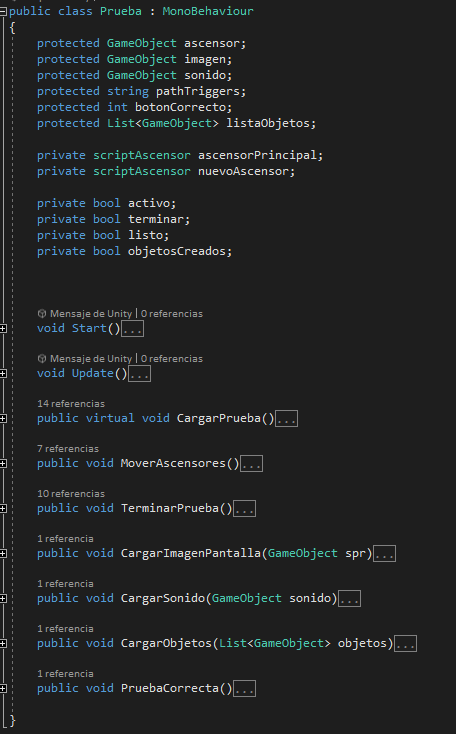
\includegraphics[width=0.5\textwidth]{04.Desarrollo/04.Entrega4/02.Iteracion4_2/00.Figuras/01.prueba.png}
    \caption{Estructura de la clase 'Prueba'.}
    \label{fig:E4_clasePrueba}
\end{figure}

\begin{figure}
  \centering
    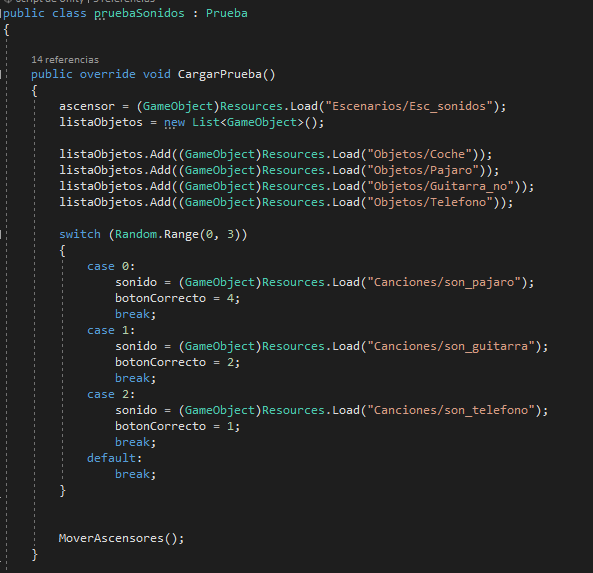
\includegraphics[width=0.7\textwidth]{04.Desarrollo/04.Entrega4/02.Iteracion4_2/00.Figuras/02.cargar_prueba.png}
    \caption{Sobrescritura del método 'CargarPrueba' para la prueba de asociación de un sonido con un objeto.}
    \label{fig:E4_cargarPrueba}
\end{figure}




\subsubsection{Pruebas de motricidad}

Para las pruebas que ejercitan la motricidad se ha utilizado la funcionalidad de los 'Triggers' creados durante el apartado \ref{E2_triggers}.

Cuando la prueba de baile da comienzo, la clase correspondiente carga la estructura de los triggers (posiciones que debe adoptar el jugador) desde un fichero JSON. También comienza a reproducir la canción requerida para la prueba correspondiente. La prueba de posiciones utiliza la misma técnica pero cargando otras estructuras diferentes y sin música, mientras que la prueba de paradas hace lo mismo pero en lugar de reproducir una canción, se prepara para reproducir un sonido que indica al jugador que tiene que detenerse.

En estas pruebas es importante la forma en la que se le transmite al usuario que posición debe adoptar. El jugador tiene que tener claro dónde tiene que colocar sus extremidades tanto vertical como horizontalmente. Un símbolo como una flecha es un icono fácilmente reconocible y con un significado muy claro si se utiliza correctamente. Teniendo en cuenta esto, un método para transmitir la información al jugador podría ser mediante flechas que aparecen delante del mismo y que indican dónde colocar las manos.

Con la idea de reflejar lo mejor posible las indicaciones al usuario, se puede utilizar una estructura que se asemeje a la propia estructura de triggers utilizada para detectar los movimientos. Mediante este paralelismo se puede mejorar la precisión y facilidad con la que el usuario capta y entiende los movimientos que tiene que hacer. De este modo, se ha creado una matriz de cuadrados con flechas que aparece frente al usuario y cambian de la misma forma que cambian los triggers (véase figura \ref{fig:E4_posiciones}).

\begin{figure}
  \centering
    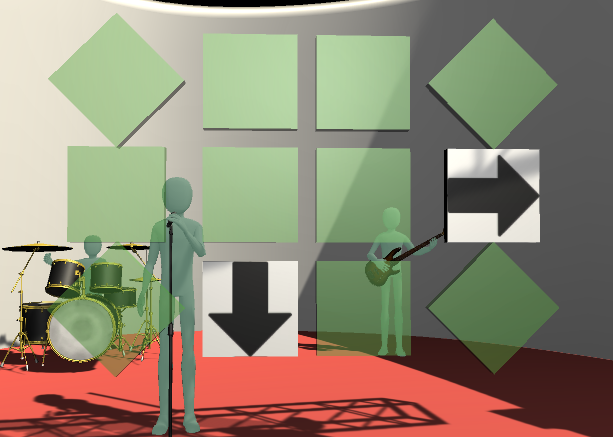
\includegraphics[width=0.7\textwidth]{04.Desarrollo/04.Entrega4/02.Iteracion4_2/00.Figuras/03.posiciones.png}
    \caption{Matriz de señales que indican al usuario dónde colocar sus manos.}
    \label{fig:E4_posiciones}
\end{figure}


\subsubsection{Pruebas de memoria}

Las pruebas de memoria se basan en presentar una imagen o canción al jugador para hacerle recordar información sobre ellas o revivir experiencias personales que tenga asociadas con ellas. Para la reproducción de las canciones se utiliza un objeto nativo de Unity llamado Audio Source. Es un objeto que permite reproducir un clip de audio dentro de la escena del juego. Por lo tanto, solo es necesario indicar qué clip de audio sonará durante cada prueba como se muestra en la figura \ref{fig:E2_audioSource}. Esta misma técnica es la que se utiliza para todas las pruebas que necesiten reproducir algún sonido.

\begin{figure}
  \centering
    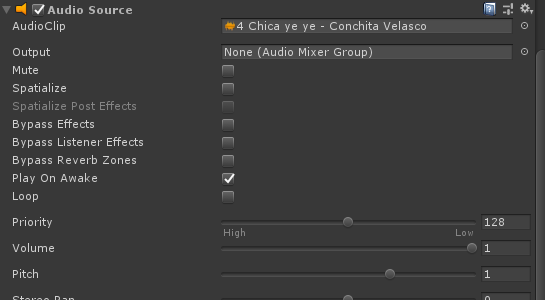
\includegraphics[width=0.7\textwidth]{04.Desarrollo/04.Entrega4/02.Iteracion4_2/00.Figuras/04.audio_source.png}
    \caption{Audio Source de Unity mostrando el clip actual que reproduce, así como otros de sus parámetros.}
    \label{fig:E4_audioSource}
\end{figure}


Para las pruebas en las que se presenta al jugador una imagen, se utiliza una primitiva de Unity que permite crear planos bidimensionales dentro de una escena 3D. Utilizando la pantalla gigante que forma parte del escenario se coloca sobre ella un plano en el que posteriormente se puede colocar como textura del mismo cualquier imagen. De esta forma, solo es necesario activar y desactivar el plano junto con su textura correspondiente. En la imagen \ref{fig:E4_imagen} se representa un objeto de tipo plano, que muestra una imagen del coliseo romano.

\begin{figure}
  \centering
    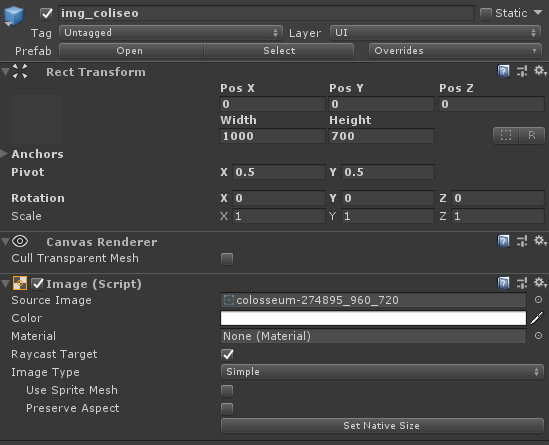
\includegraphics[width=0.7\textwidth]{04.Desarrollo/04.Entrega4/02.Iteracion4_2/00.Figuras/05.imagen.png}
    \caption{Parámetros de un objeto plano de Unity mostrando una imagen del coliseo romano.}
    \label{fig:E4_imagen}
\end{figure}


\subsubsection{Prueba de lenguaje}

En esta prueba se presenta al jugador una imagen en la que aparece una situación cotidiana, que puede haber vivido, con el objetivo de que hable y haga comentarios sobre ella. Para esto solo en necesario mostrar una imagen en la pantalla gigante del escenario, siguiendo la misma técnica usada en la prueba anterior.

\subsubsection{Pruebas de razonamiento}


Para las pruebas de razonamiento se utiliza una mesa frente al jugador en la que aparecen varios objetos con los que debe interactuar para superar el reto. En la prueba de agrupación de objetos (véase figura \ref{fig:E4_asociacion}), además es necesario crear dos zonas donde categorizar los objetos. Estas zonas pertenecen a la propia mesa y siempre son las mismas. Para cada ejemplo de esta prueba solo es necesario cambiar los objetos que se instancian. Para asegurar que todos los objetos aparecen en el lugar adecuado, se han creado cuatro objetos vacíos, asociados a la mesa, que sirven únicamente como punto de referencia. A la hora de instanciar los objetos, se buscan estas referencias y se genera un objeto en la posición de cada una. 

En la figura \ref{fig:E4_mesa} se puede ver la estructura de objeto para la mesa, que está compuesta por dos piezas (suelo y mesa), así como dos conjuntos de objetos, el primero de ellos, las 'SpawnZone' que marcan los puntos donde aparecerán los objetos; y el segundo son las plataformas donde deben colocarse los objetos para considerarse clasificados.



\begin{figure}
  \centering
    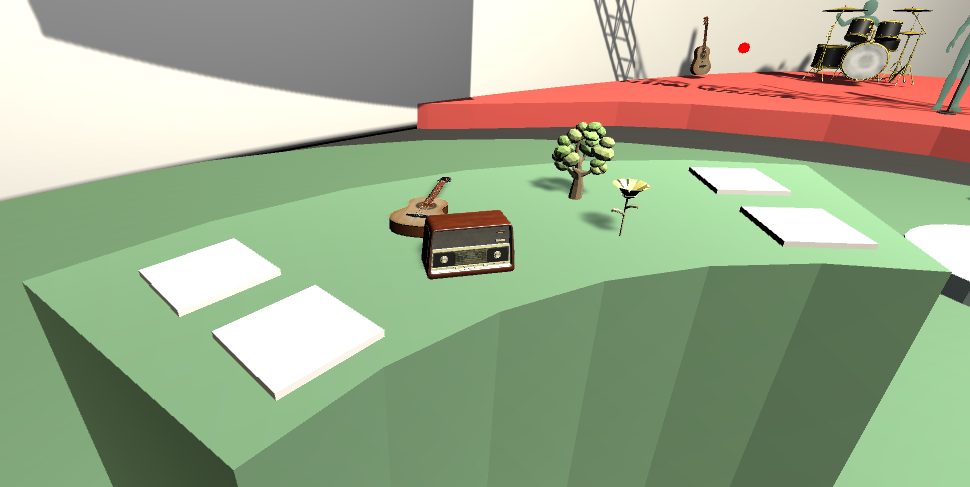
\includegraphics[width=0.7\textwidth]{04.Desarrollo/04.Entrega4/02.Iteracion4_2/00.Figuras/06.asociacion.png}
    \caption{Ejemplo de prueba de agrupación de objetos.}
    \label{fig:E4_asociacion}
\end{figure}


\begin{figure}
  \centering
    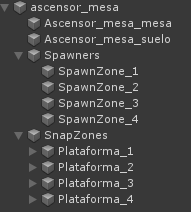
\includegraphics[width=0.4\textwidth]{04.Desarrollo/04.Entrega4/02.Iteracion4_2/00.Figuras/07.mesa.png}
    \caption{Estructura de objeto para la mesa.}
    \label{fig:E4_mesa}
\end{figure}



En la prueba de asociación de sonidos, en lugar de necesitar zonas para clasificar los objetos es necesario crear cuatro botones, uno correspondiente a cada objeto (véase figura \ref{fig:E4_sonidos}). Cada uno de estos botones puede ejecutar un método del código cuando se pulsa. Esto es lo que se utiliza para detectar la respuesta correcta, ya que en tiempo de ejecución, cuando se crean los objetos, automáticamente se asigna que el botón adecuado llame al método para dar la prueba por correcta, como se puede ver en la figura \ref{fig:E4_botonCorrecto}.


\begin{figure}
  \centering
    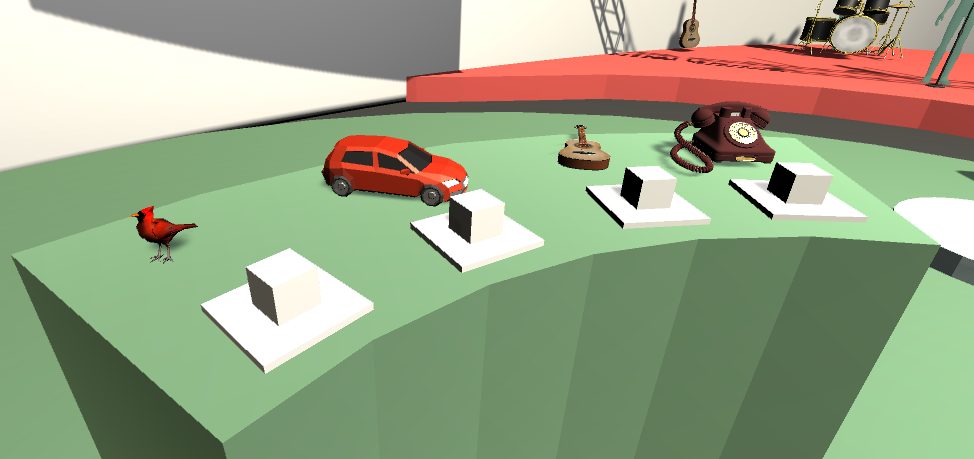
\includegraphics[width=0.7\textwidth]{04.Desarrollo/04.Entrega4/02.Iteracion4_2/00.Figuras/08.sonidos.png}
    \caption{Ejemplo de prueba de asociación de sonidos.}
    \label{fig:E4_sonidos}
\end{figure}

\begin{figure}
  \centering
    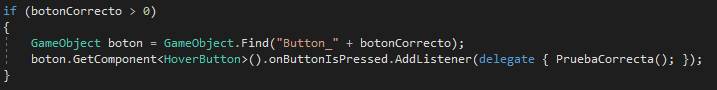
\includegraphics[width=0.9\textwidth]{04.Desarrollo/04.Entrega4/02.Iteracion4_2/00.Figuras/09.boton_correcto.png}
    \caption{Código que asigna la llamada al método para terminar la prueba de forma correcta al botón adecuado.}
    \label{fig:E4_botonCorrecto}
\end{figure}




\subsubsection{Pruebas de comprensión espacial}

Para la prueba de localización de sonidos se usa la misma técnica para la reproducción de audio usada en el resto de pruebas, pero con ligeras diferencias. En el objeto Audio Source que se encarga de reproducir el sonido, es necesario activar el parámetro 'Spatialize' (ya visto en la figura \ref{fig:E4_audioSource}), ya que es el que permite oír el sonido en 3D. La otra diferencia es que la fuente de sonido puede aparecer en cualquier punto del espacio al rededor del jugador salvo a su frente. Para esto último se generan en tiempo de ejecución tres valores en ciertos intervalos controlados para acotar el espacio posible.


